\section{Validation}\label{sec:validation}

Tests, pass criteria and expected failures were pre-registered, i.e.\ fixed before the comparisons were run. Phone
data set only one constant ($\Delta P_{\mathrm{awake}}$, \cref{sec:params}); the cell tests use their own
calibrations (V2: the HG2 cell at 25\,$^\circ$C; V4: the Oxford OCV; V5: a circuit fitted to the 1C pulses of the
DFN model). With $\varepsilon=\TTE_{\mathrm{model}}/\TTE_{\mathrm{obs}}-1$, L2 passes 31 of 59 criteria, or 28 of the
56 that are out of sample (\cref{tab:validation}).

\begin{table}[t]
\centering\footnotesize
\caption{Pre-registered tests; ``Passed'' counts criteria met by L2 (and the KiBaM variant X9).
$f_Q=Q(T)/Q(25\,^\circ\mathrm C)$ at 40/10/0/$-20\,^\circ$C, tolerance 0.05 (0.10 at $-20\,^\circ$C);
RMSE$_V$ at 40/25/10/0\,$^\circ$C (25\,$^\circ$C is the calibration temperature). In sample: the V1b idle range
and the two 25\,$^\circ$C RMSE$_V$ criteria. V3 and V4 are reported, not scored.}
\label{tab:validation}
\begin{tabular}{@{}llll@{}}
\toprule
Test & Criterion & Passed & Key result \\
\midrule
V1a Bonn & $|\varepsilon|\le 15\%$, hold-outs & 5/7 & GPS fails: $-$48\% (14 Pro), $-$20\% (13 Pro) \\
V1b Bonn & obs.\ range in 90\% UQ & 3/8 & fails: camera (13 Pro), GPS (both), camera+GPS (both) \\
V1c Bonn & additivity $\le 1\%$ & 2/2 & model +0.41\%, data +0.15\% (14 Pro) \\
V1.4 Bonn & SOC shape: D1 vs D2 & D2 & slope error D1 4.4\%, D2 2.0\% \\
V2 HG2, L2 & $|\Delta f_Q|$; RMSE$_V\le$ 50 mV & 2/8; 3/8 & $f_Q$($-$20\,\textdegree C, 2C) 0.84 vs 0.49 \\
V2 HG2, X9 & same & 4/8; 5/8 & $f_Q$($-$20\,\textdegree C, 2C) 0.52 vs 0.49 \\
V3 NASA & aged/fresh TTE & -- & $-$28.7\% vs $-$28.8\% (charge-limited) \\
V4 Oxford & RMSE$_V$ (report) & -- & 82 mV; OCV only 33 mV \\
V5 DFN, L2; X9 & $|\Delta\mathrm{TTE}|\le 3\%$, $\ge 0$\,\textdegree C & 4/6; 5/6 & L2 $\le$ 2.4\% at 25\,\textdegree C; +4.2\% at 0\,\textdegree C, 0.5C \\
V6 band & $|\varepsilon|\le 25\%$ & 11/16 & fails: Android floors, BT audio \\
V7 cold & LEE20 phenomenology & 0/3 & 0\,\textdegree C loss $-$51\% vs $-$15\% \\
\bottomrule
\end{tabular}

\end{table}

\paragraph{V1: Bonn iPhones.} Six iPhone 14 Pro and three 13 Pro units ran to empty in airplane mode with a black
screen, idle or with rear camera, GPS or both \cite{SCH26,BONN26}. Each is RP-63 with its measured capacity
(3.32, 3.16\,A\,h); the 14 Pro idle group sets $\Delta P_{\mathrm{awake}}$ and the other seven model--condition
groups are hold-outs (\cref{fig:validation_bonn}a). Idle, camera and camera+GPS are within $\pm15\,\%$ on both
phones. GPS fails ($-48$, $-20\,\%$), as pre-registered for the 14 Pro: its data imply only about 0.03\,W for GPS,
against 0.27\,W measured for a phone receiver \cite{KW19}, so the receiver in the closed box was probably
duty-cycled or without a fix. We did not retune: GPS on a stationary modern iPhone costs surprisingly little. The
90\,\% parameter interval covers only 3 of 8 observed ranges. All five misses lie above it: for GPS because of the
GPS power, otherwise because the priors of $P_{d0}$ and $\Delta P_{\mathrm{cam}}$ lie mostly above their defaults.
Camera and GPS powers add (residual $\le0.15\,\%$ in data, $\le0.43\,\%$ in model).

\emph{SOC shape.} At constant power the current rises as the OCV falls, so the coulombic display $s$ should drain
${\approx}10\,\%$ faster near empty and the energy fraction $\varsigma$ evenly. Over 28 traces the slope error is
4.4\,\% for $s$ and 2.0\,\% for $\varsigma$, and $\varsigma$ is closer on 27 of the 28 traces
(\cref{fig:validation_bonn}b): the iPhone gauge behaves as an energy gauge, so $\varsigma$ is the better display
model. Using it instead of $s$ lowers the stranded charge of the nominal cold hike by 2.2 points (44.2 to
42.0\,\%) and never by more than 2.4 points.

\begin{figure}[t]
  \centering
  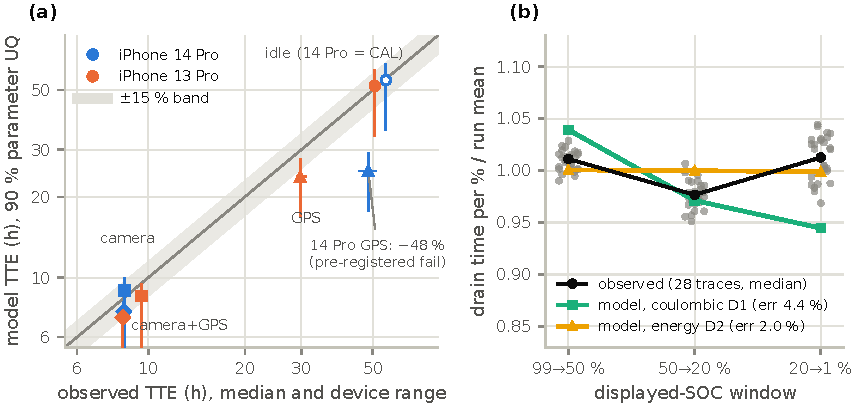
\includegraphics[width=0.88\textwidth]{figures/fig_validation_bonn.pdf}
  \caption{Bonn iPhone test. (a) Model vs.\ observed TTE with 90\,\% parameter intervals (``UQ'') and the
  $\pm15\,\%$ band (CAL: calibration run); only GPS falls outside. (b) Drain time per 1\,\% by SOC window; D1 is
  the coulombic display $s$, D2 the energy fraction $\varsigma$. The data are flat, as $\varsigma$ predicts.}
  \label{fig:validation_bonn}
\end{figure}

\paragraph{V2: temperature (LG HG2).} Calibrated at 25\,$^\circ$C only (voltage RMSE $\le34$\,mV), the LG HG2 cell
\cite{KOL20} is predicted at five other temperatures. As pre-registered, L2 under-predicts the cold loss: at
$-20\,^\circ$C it keeps 0.98 (0.5C) and 0.84 (2C) of its capacity, against 0.73 and 0.49 measured, because its
effective activation energy (about 20\,kJ/mol) is below the data's 26. The kinetic-battery variant X9
(\cref{sec:structural}) closes most of the 2C gap (0.52) but stays 0.04--0.12 high at 0.5C. Part of the loss is
not kinetic (0.90 at C/20).

\paragraph{V3, V4: aging and pulses.} V3 is only a consistency check: with NASA cell B0005's measured capacity
(1.86 to 1.33\,A\,h) and resistance growth inserted \cite{NASA07}, the 2\,A TTE falls by 28.7\,\% (observed
28.8\,\%), but both runs end by charge depletion, so TTE just scales with capacity (resistance growth alone:
0.03\,\%); the voltage RMSE is 86 and 148\,mV and the modeled temperature rise 7.1 against 14.7\,K. On an
Oxford Kokam power cell \cite{OX17} the $R\cdot Q$ scaling fails: it implies a step resistance of 84\,m$\Omega$,
four times the measured 21\,m$\Omega$, so the scaled circuit (82\,mV RMSE) fits worse than the OCV alone
(33\,mV). We therefore use the scaling only between phone packs.

\paragraph{V5: DFN reference.} Against PyBaMM's Doyle--Fuller--Newman (DFN) model \cite{SULZER21} of the Ai2020
cell \cite{AI20}, L2 is within 2.4\,\% at 25\,$^\circ$C (0.1--1C) but $+4.2\,\%$ at 0\,$^\circ$C and 0.5C, where
only X9 passes. At 1C and 0\,$^\circ$C the DFN delivers only 1.67 of 2.47\,A\,h, and at 0.5C and $-10\,^\circ$C
only 1.21: a transport-limited collapse no equivalent circuit captures (L2 $+45$ to $+364\,\%$). Sustained phone
loads ($\le0.21$C) lie between the passing and failing 0\,$^\circ$C cases.

\paragraph{V6: published runtimes.} We compare 14 published runtimes of five phones
\cite{APL14P,NBC22,NBC23,NBC24,LMAG22,GPX} at $\pm25\,\%$ (settings are undisclosed), plus two power bands
(capped gaming power and standby drain, both pass); 11 of 16 checks pass (\cref{fig:power_breakdown}b, right
column). All iPhone cases pass except Bluetooth audio ($-25.5\,\%$), which our awake-processor audio state and a
variant with audio on a low-power signal processor (X14, $+21.6\,\%$) bracket. Web browsing is within 4\,\% on
three of four phones. Android local video ($+53$, $+57\,\%$) and idle ($+54$, $+183\,\%$) fail: inverted on each
device's own battery, their runtimes imply 1.5--2.8 times our power, and we do not tune to them.

\paragraph{V7: cold shutdowns.} At or below 0\,$^\circ$C, phones shut down at 15--35\,\% displayed charge, lose
15\,\% of runtime at 0\,$^\circ$C and regain about 330\,mA\,h after warming \cite{LEE20}. For a 2015-class phone
(2.7\,A\,h, the reported 0.25\,$\Omega$ pack resistance, 3\,W bursts) the model reproduces brown-out and recovery
but overstates their size: runtime loss at 0\,$^\circ$C $-51\,\%$ (observed $-15\,\%$), shutdown at 59--78\,\%
displayed between 0 and $-10\,^\circ$C (observed 15--35\,\%) and 1430\,mA\,h recovered (observed 330). With the
0.13\,$\Omega$ resistance that the same study reports at shutdown, all three fall inside the bands ($-11\,\%$,
18\,\% at $-5\,^\circ$C, 414\,mA\,h).

\phantomsection\label{sec:wellpoor}\addcontentsline{toc}{subsection}{Where the model performs well or poorly}
\begin{keybox}[Where the model performs well or poorly]
\textbf{Well:} known loads at room temperature (Bonn idle and camera within $\pm15\,\%$, published iPhone runtimes
$-4$ to $+17\,\%$ except audio, cells within 2.4\,\% of the DFN). \textbf{Poorly:} vendor floors (the largest
cross-device uncertainty), duty-cycled GPS, and the cold, where L2 overstates capacity (V2, V5) and brown-out hinges
on pack resistance (V7). With a known floor, room-temperature TTEs hold to about $\pm15\,\%$; cold ones are indicative.
\end{keybox}
